\chapter{The Room of the Retired Baker}

The evening of the day on which the Count of Morcerf had left Danglars’
house with feelings of shame and anger at the rejection of the
projected alliance, M. Andrea Cavalcanti, with curled hair, moustaches
in perfect order, and white gloves which fitted admirably, had entered
the courtyard of the banker’s house in Rue de la Chaussée d’Antin. He
had not been more than ten minutes in the drawing-room before he drew
Danglars aside into the recess of a bow-window, and, after an ingenious
preamble, related to him all his anxieties and cares since his noble
father’s departure. He acknowledged the extreme kindness which had been
shown him by the banker’s family, in which he had been received as a
son, and where, besides, his warmest affections had found an object on
which to centre in Mademoiselle Danglars.

Danglars listened with the most profound attention; he had expected
this declaration for the last two or three days, and when at last it
came his eyes glistened as much as they had lowered on listening to
Morcerf. He would not, however, yield immediately to the young man’s
request, but made a few conscientious objections.

“Are you not rather young, M. Andrea, to think of marrying?”

“I think not, sir,” replied M. Cavalcanti; “in Italy the nobility
generally marry young. Life is so uncertain, that we ought to secure
happiness while it is within our reach.”

“Well, sir,” said Danglars, “in case your proposals, which do me honor,
are accepted by my wife and daughter, by whom shall the preliminary
arrangements be settled? So important a negotiation should, I think, be
conducted by the respective fathers of the young people.”

“Sir, my father is a man of great foresight and prudence. Thinking that
I might wish to settle in France, he left me at his departure, together
with the papers establishing my identity, a letter promising, if he
approved of my choice, 150,000 livres per annum from the day I was
married. So far as I can judge, I suppose this to be a quarter of my
father’s revenue.”

“I,” said Danglars, “have always intended giving my daughter 500,000
francs as her dowry; she is, besides, my sole heiress.”

“All would then be easily arranged if the baroness and her daughter are
willing. We should command an annuity of 175,000 livres. Supposing,
also, I should persuade the marquis to give me my capital, which is not
likely, but still is possible, we would place these two or three
millions in your hands, whose talent might make it realize ten per
cent.”

“I never give more than four per cent, and generally only three and a
half; but to my son-in-law I would give five, and we would share the
profits.”

“Very good, father-in-law,” said Cavalcanti, yielding to his low-born
nature, which would escape sometimes through the aristocratic gloss
with which he sought to conceal it. Correcting himself immediately, he
said, “Excuse me, sir; hope alone makes me almost mad,—what will not
reality do?”

“But,” said Danglars, who, on his part, did not perceive how soon the
conversation, which was at first disinterested, was turning to a
business transaction, “there is, doubtless, a part of your fortune your
father could not refuse you?”

“Which?” asked the young man.

“That you inherit from your mother.”

“Truly, from my mother, Leonora Corsinari.”

“How much may it amount to?”

“Indeed, sir,” said Andrea, “I assure you I have never given the
subject a thought, but I suppose it must have been at least two
millions.”

Danglars felt as much overcome with joy as the miser who finds a lost
treasure, or as the shipwrecked mariner who feels himself on solid
ground instead of in the abyss which he expected would swallow him up.

“Well, sir,” said Andrea, bowing to the banker respectfully, “may I
hope?”

“You may not only hope,” said Danglars, “but consider it a settled
thing, if no obstacle arises on your part.”

“I am, indeed, rejoiced,” said Andrea.

“But,” said Danglars thoughtfully, “how is it that your patron, M. de
Monte Cristo, did not make his proposal for you?”

Andrea blushed imperceptibly.

“I have just left the count, sir,” said he; “he is, doubtless, a
delightful man but inconceivably peculiar in his ideas. He esteems me
highly. He even told me he had not the slightest doubt that my father
would give me the capital instead of the interest of my property. He
has promised to use his influence to obtain it for me; but he also
declared that he never had taken on himself the responsibility of
making proposals for another, and he never would. I must, however, do
him the justice to add that he assured me if ever he had regretted the
repugnance he felt to such a step it was on this occasion, because he
thought the projected union would be a happy and suitable one. Besides,
if he will do nothing officially, he will answer any questions you
propose to him. And now,” continued he, with one of his most charming
smiles, “having finished talking to the father-in-law, I must address
myself to the banker.”

“And what may you have to say to him?” said Danglars, laughing in his
turn.

“That the day after tomorrow I shall have to draw upon you for about
four thousand francs; but the count, expecting my bachelor’s revenue
could not suffice for the coming month’s outlay, has offered me a draft
for twenty thousand francs. It bears his signature, as you see, which
is all-sufficient.”

“Bring me a million such as that,” said Danglars, “I shall be well
pleased,” putting the draft in his pocket. “Fix your own hour for
tomorrow, and my cashier shall call on you with a check for eighty
thousand francs.”

“At ten o’clock then, if you please; I should like it early, as I am
going into the country tomorrow.”

“Very well, at ten o’clock; you are still at the Hôtel des Princes?”

“Yes.”

The following morning, with the banker’s usual punctuality, the eighty
thousand francs were placed in the young man’s hands, as he was on the
point of starting, after having left two hundred francs for Caderousse.
He went out chiefly to avoid this dangerous enemy, and returned as late
as possible in the evening.

But scarcely had he stepped out of his carriage when the porter met him
with a parcel in his hand.

“Sir,” said he, “that man has been here.”

“What man?” said Andrea carelessly, apparently forgetting him whom he
but too well recollected.

“Him to whom your excellency pays that little annuity.”

“Oh,” said Andrea, “my father’s old servant. Well, you gave him the two
hundred francs I had left for him?”

“Yes, your excellency.” Andrea had expressed a wish to be thus
addressed. “But,” continued the porter, “he would not take them.”

Andrea turned pale, but as it was dark his pallor was not perceptible.
“What? he would not take them?” said he with slight emotion.

\begin{figure}[ht]
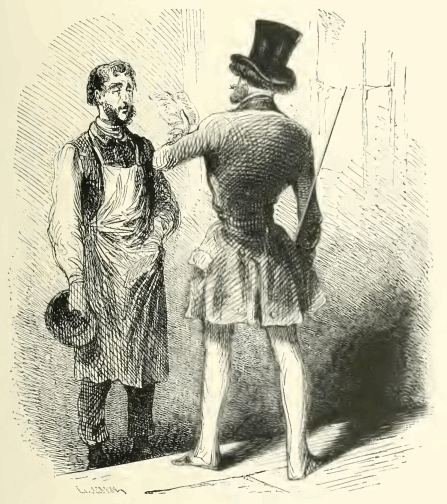
\includegraphics[width=\textwidth]{40130m.jpg}
\end{figure}

“No, he wished to speak to your excellency; I told him you were gone
out, and after some dispute he believed me and gave me this letter,
which he had brought with him already sealed.”

“Give it me,” said Andrea, and he read by the light of his
carriage-lamp:

“‘You know where I live; I expect you tomorrow morning at nine
o’clock.’”

Andrea examined it carefully, to ascertain if the letter had been
opened, or if any indiscreet eyes had seen its contents; but it was so
carefully folded, that no one could have read it, and the seal was
perfect.

“Very well,” said he. “Poor man, he is a worthy creature.” He left the
porter to ponder on these words, not knowing which most to admire, the
master or the servant.

“Take out the horses quickly, and come up to me,” said Andrea to his
groom. In two seconds the young man had reached his room and burnt
Caderousse’s letter. The servant entered just as he had finished.

“You are about my height, Pierre,” said he.

“I have that honor, your excellency.”

“You had a new livery yesterday?”

“Yes, sir.”

“I have an engagement with a pretty little girl for this evening, and
do not wish to be known; lend me your livery till tomorrow. I may
sleep, perhaps, at an inn.”

Pierre obeyed. Five minutes after, Andrea left the hotel, completely
disguised, took a cabriolet, and ordered the driver to take him to the
Cheval Rouge, at Picpus. The next morning he left that inn as he had
left the Hôtel des Princes, without being noticed, walked down the
Faubourg Saint-Antoine, along the boulevard to Rue Ménilmontant, and
stopping at the door of the third house on the left looked for someone
of whom to make inquiry in the porter’s absence.

“For whom are you looking, my fine fellow?” asked the fruiteress on the
opposite side.

“Monsieur Pailletin, if you please, my good woman,” replied Andrea.

“A retired baker?” asked the fruiteress.

“Exactly.”

“He lives at the end of the yard, on the left, on the third story.”

\begin{figure}[ht]
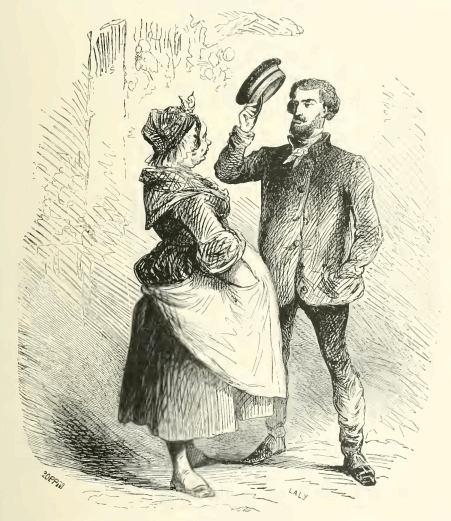
\includegraphics[width=\textwidth]{40132m.jpg}
\end{figure}

Andrea went as she directed him, and on the third floor he found a
hare’s paw, which, by the hasty ringing of the bell, it was evident he
pulled with considerable ill-temper. A moment after Caderousse’s face
appeared at the grating in the door.

“Ah! you are punctual,” said he, as he drew back the door.

“Confound you and your punctuality!” said Andrea, throwing himself into
a chair in a manner which implied that he would rather have flung it at
the head of his host.

“Come, come, my little fellow, don’t be angry. See, I have thought
about you—look at the good breakfast we are going to have; nothing but
what you are fond of.”

Andrea, indeed, inhaled the scent of something cooking which was not
unwelcome to him, hungry as he was; it was that mixture of fat and
garlic peculiar to Provençal kitchens of an inferior order, added to
that of dried fish, and above all, the pungent smell of musk and
cloves. These odors escaped from two deep dishes which were covered and
placed on a stove, and from a copper pan placed in an old iron pot. In
an adjoining room Andrea saw also a tolerably clean table prepared for
two, two bottles of wine sealed, the one with green, the other with
yellow, a supply of brandy in a decanter, and a measure of fruit in a
cabbage-leaf, cleverly arranged on an earthenware plate.

“What do you think of it, my little fellow?” said Caderousse. “Ay, that
smells good! You know I used to be a good cook; do you recollect how
you used to lick your fingers? You were among the first who tasted any
of my dishes, and I think you relished them tolerably.” While speaking,
Caderousse went on peeling a fresh supply of onions.

“But,” said Andrea, ill-temperedly, “by my faith, if it was only to
breakfast with you, that you disturbed me, I wish the devil had taken
you!”

“My boy,” said Caderousse sententiously, “one can talk while eating.
And then, you ungrateful being, you are not pleased to see an old
friend? I am weeping with joy.”

He was truly crying, but it would have been difficult to say whether
joy or the onions produced the greatest effect on the lachrymal glands
of the old innkeeper of the Pont-du-Gard.

“Hold your tongue, hypocrite,” said Andrea; “you love me!”

“Yes, I do, or may the devil take me. I know it is a weakness,” said
Caderousse, “but it overpowers me.”

“And yet it has not prevented your sending for me to play me some
trick.”

“Come,” said Caderousse, wiping his large knife on his apron, “if I did
not like you, do you think I should endure the wretched life you lead
me? Think for a moment. You have your servant’s clothes on—you
therefore keep a servant; I have none, and am obliged to prepare my own
meals. You abuse my cookery because you dine at the table d’hôte of the
Hôtel des Princes, or the Café de Paris. Well, I too could keep a
servant; I too could have a tilbury; I too could dine where I like; but
why do I not? Because I would not annoy my little Benedetto. Come, just
acknowledge that I could, eh?”

This address was accompanied by a look which was by no means difficult
to understand.

“Well,” said Andrea, “admitting your love, why do you want me to
breakfast with you?”

“That I may have the pleasure of seeing you, my little fellow.”

“What is the use of seeing me after we have made all our arrangements?”

“Eh, dear friend,” said Caderousse, “are wills ever made without
codicils? But you first came to breakfast, did you not? Well, sit down,
and let us begin with these pilchards, and this fresh butter; which I
have put on some vine-leaves to please you, wicked one. Ah, yes; you
look at my room, my four straw chairs, my images, three francs each.
But what do you expect? This is not the Hôtel des Princes.”

“Come, you are growing discontented, you are no longer happy; you, who
only wish to live like a retired baker.”

Caderousse sighed.

“Well, what have you to say? you have seen your dream realized.”

“I can still say it is a dream; a retired baker, my poor Benedetto, is
rich—he has an annuity.”

“Well, you have an annuity.”

“I have?”

\begin{figure}[ht]
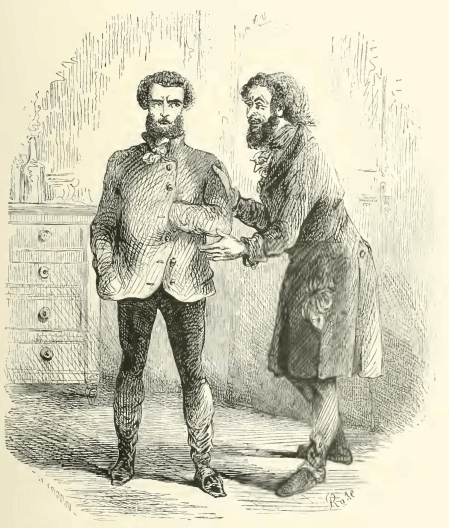
\includegraphics[width=\textwidth]{40134m.jpg}
\end{figure}

“Yes, since I bring you your two hundred francs.”

Caderousse shrugged his shoulders.

“It is humiliating,” said he, “thus to receive money given
grudgingly,—an uncertain supply which may soon fail. You see I am
obliged to economize, in case your prosperity should cease. Well, my
friend, fortune is inconstant, as the chaplain of the regiment said. I
know your prosperity is great, you rascal; you are to marry the
daughter of Danglars.”

“What? of Danglars?”

“Yes, to be sure; must I say Baron Danglars? I might as well say Count
Benedetto. He was an old friend of mine and if he had not so bad a
memory he ought to invite me to your wedding, seeing he came to mine.
Yes, yes, to mine; gad, he was not so proud then,—he was an under-clerk
to the good M. Morrel. I have dined many times with him and the Count
of Morcerf, so you see I have some high connections and were I to
cultivate them a little, we might meet in the same drawing-rooms.”

“Come, your jealousy represents everything to you in the wrong light.”

“That is all very fine, Benedetto mio, but I know what I am saying.
Perhaps I may one day put on my best coat, and presenting myself at the
great gate, introduce myself. Meanwhile let us sit down and eat.”

Caderousse set the example and attacked the breakfast with good
appetite, praising each dish he set before his visitor. The latter
seemed to have resigned himself; he drew the corks, and partook largely
of the fish with the garlic and fat.

“Ah, mate,” said Caderousse, “you are getting on better terms with your
old landlord!”

“Faith, yes,” replied Andrea, whose hunger prevailed over every other
feeling.

“So you like it, you rogue?”

“So much that I wonder how a man who can cook thus can complain of hard
living.”

“Do you see,” said Caderousse, “all my happiness is marred by one
thought?”

“What is that?”

“That I am dependent on another, I who have always gained my own
livelihood honestly.”

“Do not let that disturb you, I have enough for two.”

“No, truly; you may believe me if you will; at the end of every month I
am tormented by remorse.”

“Good Caderousse!”

“So much so, that yesterday I would not take the two hundred francs.”

“Yes, you wished to speak to me; but was it indeed remorse, tell me?”

“True remorse; and, besides, an idea had struck me.”

Andrea shuddered; he always did so at Caderousse’s ideas.

“It is miserable—do you see?—always to wait till the end of the month.”

“Oh,” said Andrea philosophically, determined to watch his companion
narrowly, “does not life pass in waiting? Do I, for instance, fare
better? Well, I wait patiently, do I not?”

“Yes; because instead of expecting two hundred wretched francs, you
expect five or six thousand, perhaps ten, perhaps even twelve, for you
take care not to let anyone know the utmost. Down there, you always had
little presents and Christmas-boxes, which you tried to hide from your
poor friend Caderousse. Fortunately he is a cunning fellow, that friend
Caderousse.”

“There you are beginning again to ramble, to talk again and again of
the past! But what is the use of teasing me with going all over that
again?”

“Ah, you are only one-and-twenty, and can forget the past; I am fifty,
and am obliged to recollect it. But let us return to business.”

“Yes.”

“I was going to say, if I were in your place——”

“Well.”

“I would realize——”

“How would you realize?”

“I would ask for six months’ in advance, under pretence of being able
to purchase a farm, then with my six months I would decamp.”

“Well, well,” said Andrea, “that isn’t a bad idea.”

“My dear friend,” said Caderousse, “eat of my bread, and take my
advice; you will be none the worse off, physically or morally.”

“But,” said Andrea, “why do you not act on the advice you gave me? Why
do you not realize a six months’, a year’s advance even, and retire to
Brussels? Instead of living the retired baker, you might live as a
bankrupt, using his privileges; that would be very good.”

“But how the devil would you have me retire on twelve hundred francs?”

“Ah, Caderousse,” said Andrea, “how covetous you are! Two months ago
you were dying with hunger.”

“The appetite grows by what it feeds on,” said Caderousse, grinning and
showing his teeth, like a monkey laughing or a tiger growling. “And,”
added he, biting off with his large white teeth an enormous mouthful of
bread, “I have formed a plan.”

Caderousse’s plans alarmed Andrea still more than his ideas; ideas were
but the germ, the plan was reality.

“Let me see your plan; I dare say it is a pretty one.”

“Why not? Who formed the plan by which we left the establishment of
M——! eh? was it not I? and it was no bad one I believe, since here we
are!”

“I do not say,” replied Andrea, “that you never make a good one; but
let us see your plan.”

“Well,” pursued Caderousse, “can you without expending one sou, put me
in the way of getting fifteen thousand francs? No, fifteen thousand are
not enough,—I cannot again become an honest man with less than thirty
thousand francs.”

“No,” replied Andrea, dryly, “no, I cannot.”

“I do not think you understand me,” replied Caderousse, calmly; “I said
without your laying out a sou.”

“Do you want me to commit a robbery, to spoil all my good fortune—and
yours with mine—and both of us to be dragged down there again?”

“It would make very little difference to me,” said Caderousse, “if I
were retaken, I am a poor creature to live alone, and sometimes pine
for my old comrades; not like you, heartless creature, who would be
glad never to see them again.”

Andrea did more than tremble this time, he turned pale.

“Come, Caderousse, no nonsense!” said he.

“Don’t alarm yourself, my little Benedetto, but just point out to me
some means of gaining those thirty thousand francs without your
assistance, and I will contrive it.”

“Well, I’ll see—I’ll try to contrive some way,” said Andrea.

“Meanwhile you will raise my monthly allowance to five hundred francs,
my little fellow? I have a fancy, and mean to get a housekeeper.”

“Well, you shall have your five hundred francs,” said Andrea; “but it
is very hard for me, my poor Caderousse—you take advantage——”

“Bah,” said Caderousse, “when you have access to countless stores.”

One would have said Andrea anticipated his companion’s words, so did
his eye flash like lightning, but it was but for a moment.

“True,” he replied, “and my protector is very kind.”

“That dear protector,” said Caderousse; “and how much does he give you
monthly?”

“Five thousand francs.”

“As many thousands as you give me hundreds! Truly, it is only bastards
who are thus fortunate. Five thousand francs per month! What the devil
can you do with all that?”

“Oh, it is no trouble to spend that; and I am like you, I want
capital.”

“Capital?—yes—I understand—everyone would like capital.”

“Well, and I shall get it.”

“Who will give it to you—your prince?”

“Yes, my prince. But unfortunately I must wait.”

\begin{figure}[ht]
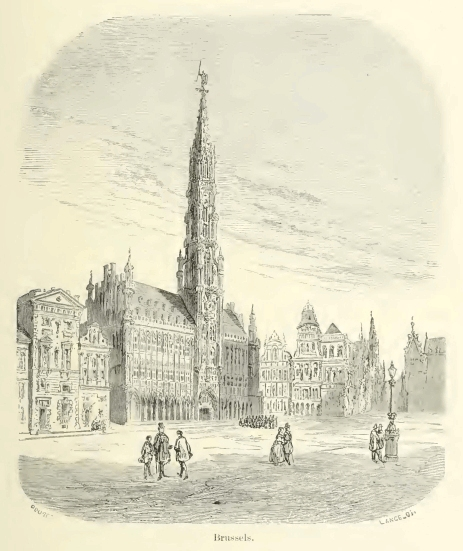
\includegraphics[width=\textwidth]{40138m.jpg}
\end{figure}

“You must wait for what?” asked Caderousse.

“For his death.”

“The death of your prince?”

“Yes.”

“How so?”

“Because he has made his will in my favor.”

“Indeed?”

“On my honor.”

“For how much?”

“For five hundred thousand.”

“Only that? It’s little enough.”

“But so it is.”

“No, it cannot be!”

“Are you my friend, Caderousse?”

“Yes, in life or death.”

“Well, I will tell you a secret.”

“What is it?”

“But remember——”

“Ah! \textit{pardieu!} mute as a carp.”

“Well, I think——”

Andrea stopped and looked around.

“You think? Do not fear; \textit{pardieu!} we are alone.”

“I think I have discovered my father.”

“Your true father?”

“Yes.”

“Not old Cavalcanti?”

“No, for he has gone again; the true one, as you say.”

“And that father is——”

“Well, Caderousse, it is Monte Cristo.”

“Bah!”

“Yes, you understand, that explains all. He cannot acknowledge me
openly, it appears, but he does it through M. Cavalcanti, and gives him
fifty thousand francs for it.”

“Fifty thousand francs for being your father? I would have done it for
half that, for twenty thousand, for fifteen thousand; why did you not
think of me, ungrateful man?”

“Did I know anything about it, when it was all done when I was down
there?”

“Ah, truly? And you say that by his will——”

“He leaves me five hundred thousand livres.”

“Are you sure of it?”

“He showed it me; but that is not all—there is a codicil, as I said
just now.”

“Probably.”

“And in that codicil he acknowledges me.”

“Oh, the good father, the brave father, the very honest father!” said
Caderousse, twirling a plate in the air between his two hands.

“Now, say if I conceal anything from you?”

“No, and your confidence makes you honorable in my opinion; and your
princely father, is he rich, very rich?”

“Yes, he is that; he does not himself know the amount of his fortune.”

“Is it possible?”

“It is evident enough to me, who am always at his house. The other day
a banker’s clerk brought him fifty thousand francs in a portfolio about
the size of your plate; yesterday his banker brought him a hundred
thousand francs in gold.”

Caderousse was filled with wonder; the young man’s words sounded to him
like metal, and he thought he could hear the rushing of cascades of
louis.

“And you go into that house?” cried he briskly.

“When I like.”

Caderousse was thoughtful for a moment. It was easy to perceive he was
revolving some unfortunate idea in his mind. Then suddenly,—

“How I should like to see all that,” cried he; “how beautiful it must
be!”

“It is, in fact, magnificent,” said Andrea.

“And does he not live in the Champs-Élysées?”

“Yes, No. 30.”

“Ah,” said Caderousse, “No. 30.”

“Yes, a fine house standing alone, between a courtyard and a
garden,—you must know it.”

“Possibly; but it is not the exterior I care for, it is the interior.
What beautiful furniture there must be in it!”

“Have you ever seen the Tuileries?”

“No.”

“Well, it surpasses that.”

“It must be worth one’s while to stoop, Andrea, when that good M. Monte
Cristo lets fall his purse.”

“It is not worthwhile to wait for that,” said Andrea; “money is as
plentiful in that house as fruit in an orchard.”

“But you should take me there one day with you.”

“How can I? On what plea?”

“You are right; but you have made my mouth water. I must absolutely see
it; I shall find a way.”

“No nonsense, Caderousse!”

“I will offer myself as floor-polisher.”

“The rooms are all carpeted.”

“Well, then, I must be contented to imagine it.”

“That is the best plan, believe me.”

“Try, at least, to give me an idea of what it is.”

“How can I?”

“Nothing is easier. Is it large?”

“Middling.”

“How is it arranged?”

“Faith, I should require pen, ink, and paper to make a plan.”

“They are all here,” said Caderousse, briskly. He fetched from an old
secretaire a sheet of white paper and pen and ink. “Here,” said
Caderousse, “draw me all that on the paper, my boy.”

Andrea took the pen with an imperceptible smile and began.

“The house, as I said, is between the court and the garden; in this
way, do you see?” Andrea drew the garden, the court and the house.

\begin{figure}[ht]
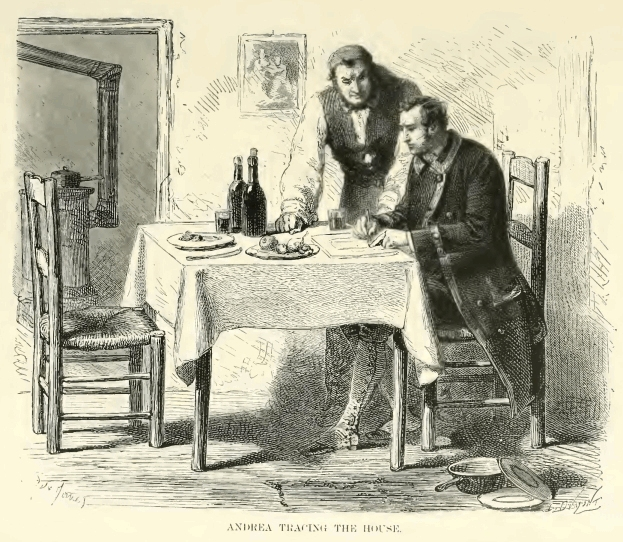
\includegraphics[width=\textwidth]{40142m.jpg}
\end{figure}

“High walls?”

“Not more than eight or ten feet.”

“That is not prudent,” said Caderousse.

“In the court are orange-trees in pots, turf, and clumps of flowers.”

“And no steel-traps?”

“No.”

“The stables?”

“Are on either side of the gate, which you see there.” And Andrea
continued his plan.

“Let us see the ground floor,” said Caderousse.

“On the ground floor, dining-room, two drawing-rooms, billiard-room,
staircase in the hall, and a little back staircase.”

“Windows?”

“Magnificent windows, so beautiful, so large, that I believe a man of
your size should pass through each frame.”

“Why the devil have they any stairs with such windows?”

“Luxury has everything.”

“But shutters?”

“Yes, but they are never used. That Count of Monte Cristo is an
original, who loves to look at the sky even at night.”

“And where do the servants sleep?”

“Oh, they have a house to themselves. Picture to yourself a pretty
coach-house at the right-hand side where the ladders are kept. Well,
over that coach-house are the servants’ rooms, with bells corresponding
with the different apartments.”

“Ah, \textit{diable!} bells did you say?”

“What do you mean?”

“Oh, nothing! I only say they cost a load of money to hang, and what is
the use of them, I should like to know?”

“There used to be a dog let loose in the yard at night, but it has been
taken to the house at Auteuil, to that you went to, you know.”

“Yes.”

“I was saying to him only yesterday, ‘You are imprudent, Monsieur
Count; for when you go to Auteuil and take your servants the house is
left unprotected.’ ‘Well,’ said he, ‘what next?’ ‘Well, next, some day
you will be robbed.’”

“What did he answer?”

“He quietly said, ‘What do I care if I am?’”

“Andrea, he has some secretaire with a spring.”

“How do you know?”

“Yes, which catches the thief in a trap and plays a tune. I was told
there were such at the last exhibition.”

“He has simply a mahogany secretaire, in which the key is always kept.”

“And he is not robbed?”

“No; his servants are all devoted to him.”

“There ought to be some money in that secretaire?”

“There may be. No one knows what there is.”

“And where is it?”

“On the first floor.”

“Sketch me the plan of that floor, as you have done of the ground
floor, my boy.”

“That is very simple.” Andrea took the pen. “On the first story, do you
see, there is the anteroom and the drawing-room; to the right of the
drawing-room, a library and a study; to the left, a bedroom and a
dressing-room. The famous secretaire is in the dressing-room.”

“Is there a window in the dressing-room?”

“Two,—one here and one there.” Andrea sketched two windows in the room,
which formed an angle on the plan, and appeared as a small square added
to the rectangle of the bedroom. Caderousse became thoughtful.

“Does he often go to Auteuil?” added he.

“Two or three times a week. Tomorrow, for instance, he is going to
spend the day and night there.”

“Are you sure of it?”

“He has invited me to dine there.”

“There’s a life for you,” said Caderousse; “a town house and a country
house.”

“That is what it is to be rich.”

“And shall you dine there?”

“Probably.”

“When you dine there, do you sleep there?”

“If I like; I am at home there.”

Caderousse looked at the young man, as if to get at the truth from the
bottom of his heart. But Andrea drew a cigar-case from his pocket, took
a Havana, quietly lit it, and began smoking.

“When do you want your twelve hundred francs?” said he to Caderousse.

“Now, if you have them.” Andrea took five-and-twenty louis from his
pocket.

“Yellow boys?” said Caderousse; “no, I thank you.”

“Oh, you despise them.”

“On the contrary, I esteem them, but will not have them.”

“You can change them, idiot; gold is worth five sous.”

“Exactly; and he who changes them will follow friend Caderousse, lay
hands on him, and demand what farmers pay him their rent in gold. No
nonsense, my good fellow; silver simply, round coins with the head of
some monarch or other on them. Anybody may possess a five-franc piece.”

“But do you suppose I carry five hundred francs about with me? I should
want a porter.”

“Well, leave them with your porter; he is to be trusted. I will call
for them.”

“Today?”

“No, tomorrow; I shall not have time today.”

“Well, tomorrow I will leave them when I go to Auteuil.”

“May I depend on it?”

“Certainly.”

“Because I shall secure my housekeeper on the strength of it.”

“Now see here, will that be all? Eh? And will you not torment me any
more?”

“Never.”

Caderousse had become so gloomy that Andrea feared he should be obliged
to notice the change. He redoubled his gayety and carelessness.

“How sprightly you are,” said Caderousse; “One would say you were
already in possession of your property.”

“No, unfortunately; but when I do obtain it——”

“Well?”

“I shall remember old friends, I can tell you that.”

“Yes, since you have such a good memory.”

“What do you want? It looks as if you were trying to fleece me?”

“I? What an idea! I, who am going to give you another piece of good
advice.”

“What is it?”

“To leave behind you the diamond you have on your finger. We shall both
get into trouble. You will ruin both yourself and me by your folly.”

“How so?” said Andrea.

“How? You put on a livery, you disguise yourself as a servant, and yet
keep a diamond on your finger worth four or five thousand francs.”

“You guess well.”

“I know something of diamonds; I have had some.”

“You do well to boast of it,” said Andrea, who, without becoming angry,
as Caderousse feared, at this new extortion, quietly resigned the ring.
Caderousse looked so closely at it that Andrea well knew that he was
examining to see if all the edges were perfect.

“It is a false diamond,” said Caderousse.

“You are joking now,” replied Andrea.

“Do not be angry, we can try it.” Caderousse went to the window,
touched the glass with it, and found it would cut.

“\textit{Confiteor!}” said Caderousse, putting the diamond on his little
finger; “I was mistaken; but those thieves of jewellers imitate so well
that it is no longer worthwhile to rob a jeweller’s shop—it is another
branch of industry paralyzed.”

“Have you finished?” said Andrea,—“do you want anything more?—will you
have my waistcoat or my hat? Make free, now you have begun.”

“No; you are, after all, a good companion; I will not detain you, and
will try to cure myself of my ambition.”

“But take care the same thing does not happen to you in selling the
diamond you feared with the gold.”

“I shall not sell it—do not fear.”

“Not at least till the day after tomorrow,” thought the young man.

“Happy rogue,” said Caderousse; “you are going to find your servants,
your horses, your carriage, and your betrothed!”

“Yes,” said Andrea.

“Well, I hope you will make a handsome wedding-present the day you
marry Mademoiselle Danglars.”

“I have already told you it is a fancy you have taken in your head.”

“What fortune has she?”

“But I tell you——”

“A million?”

Andrea shrugged his shoulders.

“Let it be a million,” said Caderousse; “you can never have so much as
I wish you.”

“Thank you,” said the young man.

“Oh, I wish it you with all my heart!” added Caderousse with his hoarse
laugh. “Stop, let me show you the way.”

“It is not worthwhile.”

“Yes, it is.”

“Why?”

“Because there is a little secret, a precaution I thought it desirable
to take, one of Huret \& Fichet’s locks, revised and improved by Gaspard
Caderousse; I will manufacture you a similar one when you are a
capitalist.”

“Thank you,” said Andrea; “I will let you know a week beforehand.”

They parted. Caderousse remained on the landing until he had not only
seen Andrea go down the three stories, but also cross the court. Then
he returned hastily, shut his door carefully, and began to study, like
a clever architect, the plan Andrea had left him.

“Dear Benedetto,” said he, “I think he will not be sorry to inherit his
fortune, and he who hastens the day when he can touch his five hundred
thousand will not be his worst friend.”
